
\chapter{Ideal adapter modeling methods and assumptions}\label{chap:ideal-adapter-appendix}

This appendix lays out the basic Bayesian belief updating model proposed as part of the ideal adapter framework. %Section~\ref{sec:ideal-adapter}
% Appendix~\ref{sec:model-fitting-methods} summarizes
We first summarize the formal specification of the model. As we describe in the main text, the model assumes that adaptation takes place over a cue dimension that might integrate auditory and visual information. The arguments for this assumption, potential caveats, and our reply to those caveats are summarized
% in Appendix~\ref{sec:audio-visual-cue}.
next. We then %Appendix~\ref{sec:model-fitt-param}
describe how the model's parameters were fit to the behavioral data from \textcite{Vroomen2007} and our own study. Throughout these sections we state the assumptions made by our model and model fitting procedure. Crucially, none of these assumptions creates a bias in favor of our hypothesis. Finally, we provide a table that summarizes our assumptions.
% is provided in a Appendix~\ref{sec:model-assumptions}.

\section{Model specification}
\label{sec:model-fitting-methods}

To quantify and test the qualitative predictions of the ideal adapter framework, we implemented a basic Bayesian belief updating model.  This model makes a number of simplifying assumptions. The most notable is that we consider only two categories in this model, \ph b and \ph d, and assume that the prior beliefs about their means and variances are independent
\begin{equation}
  \label{eq:21}
  p(\boldsymbol{\mu, \sigma}^2) = \prod_c p(\mu_c, \sigma^2_c) = p(\mu_\mrb, \sigma^2_\mrb, \mu_\mrd, \sigma^2_\mrd)
\end{equation}
Combined with the fact that participants in these experiments reliably classify even the auditorily ambiguous audio-visual adaptors as the intended categories \autocite{Vroomen2004}, this simplifies belief updating (Equation~\ref{eq:10}).

The form of the individual category parameter priors was also chosen for reasons of computational convenience.  We use the conjugate prior for the Normal distribution with unknown mean and variance, a Normal-$\chi^{-2}$ distribution \autocite{Gelman2003}.  This distribution factorizes the joint prior into two components:
\begin{align}
  \label{eq:7}
  p(\mu_c, \sigma^2_c) &= p(\mu_c \given \sigma^2_c) p(\sigma^2_c)\\
  &= \mathrm{Normal} (\mu_c \given \mu_{0,c}, \sigma^2_c / \kappa_0) \chi^{-2} (\sigma^2_c \given \nu_0, \sigma^2_{c,0})
\end{align}
The prior on the variance is a $\chi^{-2}$ distribution, with two parameters, $\nu_0$ and $\sigma^2_{c,0}$.  $\sigma^2_{c,0}$  is the expected value of the category variance $\sigma^2_c$, while $\nu_0$ represents the effective prior sample size for the mean (reflecting the uncertainty about $\sigma^2_{c,0}$, see main text)%, Section \ref{sec:bayes-beli-updat}).
The prior on the mean is conditioned on the value of the category variance, and is a Normal distribution. The expected value of that normal distribution is the prior mean parameter $\mu_{0,c}$. Its variance is $\sigma^2_c / \kappa_0$, i.e., the \emph{category} variance divided by the effective prior sample size for the mean $\kappa_0$.

\subsection{Belief updating with a conjugate prior}
\label{sec:belief-updating-with}

Using a conjugate prior is convenient because after updating with observations $X = x_1, \ldots, x_n$ (whose mean value is $\bar x$ and sample variance is $s^2 = \frac{1}{n} \sum_i (x_i - \bar x)^2$), the posterior is \emph{also} a Normal-$\chi^{-2}$ distribution, with updated parameters \autocite{Gelman2003}:
\begin{align}
  \label{eq:8}
  \kappa_n &= \kappa_0 + n \\
  \mu_{n,c} &= \frac{\kappa_0}{\kappa_n} \mu_{0,c} + \frac{n}{\kappa_n} \bar x \\
  \nu_n &= \nu_0 + n \\
  \sigma^2_{n,c} &= \frac{1}{\nu_n} ( \nu_0 \sigma^2_{c,0} + n s^2 + \frac{n \kappa_0}{\kappa_n} (\mu_{0,c} - \bar x)^2 )  \label{eq:post-sum-of-squares}
\end{align}
These parameter updates have intuitive interpretations: the $\kappa_0$ and $\nu_0$ parameters are `pseudocounts', or the effective sample size of the prior.  To update them from their prior to posterior values, they are both incremented by $n$, the number of observations.  The updated mean $\mu_{n,c}$ is a weighted average of the sample mean (weighted by the actual sample size $n$) and the prior mean (weighted by the prior effective sample size of the mean $\kappa_0$).  The updated expected variance $\sigma^2_{n,c}$ is also a weighted average, of the observed variance $n s^2$ (weighted by the actual sample size $n$), the prior expected variance $\sigma^2_{0,c}$ (weighted by the effective prior sample size, $\nu_0$), and a third term, which accounts for deviation of the observed mean from the expected mean $\mu_{c,0}$.  This last term is weighted by $n \kappa_0 / \kappa_n$, which gets larger (relative to the weights of the other terms, $n$ and $\nu_0$) when $n \approx \kappa_0$.

What happens to the expected mean and variance when more and more observations are made?  Specifically, what happens when $n$ becomes much larger than the prior effective sample sizes for the variance $\nu_0$ and mean $\kappa_0$?  First, the posterior mean $\mu_n$ converges to the observed mean $\bar x$ (since $n/\kappa_n = n/(\kappa_0+n) \approx 1$ when $n \gg \kappa_0$).  Second, and similarly, the expected variance converges on the observed variance. That is, with a lot of data about the current situation the model's beliefs will converge against the actual statistics of that situation. In both cases, the stronger the prior beliefs (larger prior sample sizes $\kappa_0$ and $\nu_0$), the more observations it takes to overcome the listener's prior beliefs.  These prior effective sample size parameters can thus be understood as controlling the strength and speed of adaptation effects.

\subsection{Incremental belief updating}
\label{sec:incr-beli-updat}

If all the individual, observed cue values for each category are assumed to be statistically independent (conditioned on the mean and variance), then the joint likelihood of all observed cues is equal to the product of the individual likelihoods, and thus
\begin{align}
  \label{eq:6}
  p(\mu_c, \sigma^2_c \given x_1 \ldots x_N) &\propto \underbrace{p(x_1, \ldots, x_N \given \mu_c, \sigma^2_c)}_{\mathrm{joint\ likelihood}} \underbrace{p(\mu_c, \sigma^2_c)}_{\mathrm{prior}} \\
  &\propto \left( \prod_{i=1}^N p(x_i \given \mu_c, \sigma^2_c)  \right) p(\mu_c, \sigma^2_c) \\
  &\propto p(x_N \given \mu_c, \sigma^2_c) \left( \prod_{i=1}^{N-1} p(x_i \given \mu_c, \sigma^2_c)  \right) p(\mu_c, \sigma^2_c) \\
  &\propto \underbrace{p(x_N \given \mu_c, \sigma^2_c)}_{\mathrm{likelihood\ of\ }x_N} \underbrace{p(\mu_c, \sigma^2_c \given x_1, \ldots, x_{N-1})}_{\mathrm{updated\ prior}}
\end{align}
That is, the listener's beliefs after the $N$th observation are a combination of their beliefs about the means and variances after all $N-1$ preceding observations, combined with the likelihood of the current observation given those beliefs.

One insight this provides is that it is not always necessary to maintain a full record of all observations made so far, or even their statistics.  Rather, it is sufficient to just track the posterior distribution over means and variances after each token.  This leads naturally to approximate inference methods like particle filters, which approximate beliefs after $N-1$ observations via a set of ``particles'', each a particular set of means and variances, with the particles collectively approximating the full distribution $p(\mu_c, \sigma^2_c)$.  After observation $N$, each particle's estimate is updated, with particles failing to predict observation $N$ effectively being thrown out and particles which do effectively predict observation $N$ persisting or even being ``cloned'' to replace the rejected particles.  Particle filters have been shown to be a reasonable approximation of Bayes-optimal inference in distributional learning categorization problems, and match human performance well even with a small number of particles \autocite{Sanborn2010}.

\section{Audio-visual cue integration}
\label{sec:audio-visual-cue}

Next, we discuss the model's assumptions about the nature of the dimension over which adaptation takes place. This part of the model is not a consequences of the ideal adapter framework. Instead, it is motivated by evidence for cross-modal interactions in audio-visual speech processing \autocite{Bejjanki2011,McGurk1976}. Given evidence for such cross-modal interactions, we remain agnostic about the level at which listeners are adapting to the audio-visual stimuli. Specifically, we treat as a free parameter whether listeners adapt to a purely auditory representation of the perceived cues, or to some representation which integrates information from both auditory and visual cues. After describing how this was implemented in the model, we summarize possible objections to this aspect of the model and our reply to these objections.

\subsection{Linear cue combination}
\label{sec:line-cue-comb}

Under reasonably general assumptions, information from auditory and visual cues to the same phonetic dimension can be optimally combined into a multimodal cue value by a weighted sum $x=w_a x^{(a)} + w_v x^{(v)}$, where the weights $w_a$ and $w_v$ sum to 1 and are proportional to the reliability of the auditory and visual cues \autocite{Bejjanki2011,Ernst2002,Jacobs2002,Knill2003,Toscano2010}.

We incorporate this into our model via treating the perceived cue values $x$ as a weighted sum of the continuum values for the auditory and visual tokens $x=wx^{(v)} + (1-w)x^{(a)}$, where the weight $w$ is a free parameter.  For the audio-visual adaptors used in this experiment, in the \ph b condition the visual cue indicates a prototypical \ph b, and so $x^{(v)} = 1$, while the auditory cue indicates an ambiguous \ph b-\ph d, $x^{(a)} = x_\mathrm{bd} \approx 5$ (depending on the particular participant's most ambiguous stimulus).

The linear combination of these two cues results in an integrated cue estimate somewhere in between, not quite prototypical but not fully ambiguous.  Note that for our model fits, the best-fitting cue weights are in general roughly equal ($w\approx 0.5$), which suggests that the perceived cue value for the audiovisual adaptor is substantially less ambiguous than the auditory cue. This is hardly surprising given well-known cross-modal effects on speech perception with similar consequences, such as the McGurk effect \autocite{McGurk1976}.
The assumption that the audio-visual stimulus is  not really ambiguous is also consistent with our finding from pilot studies that participants can reliably classify the ambiguous audiovisual adaptor stimuli (which also justifies somewhat our assumption---made solely for the sake of convenience---that the category label of each adaptor stimulus is known with certainty).

\subsection{Is there evidence against audio-visual integration in adaptation?}
\label{sec:evid-against-audio}

Our decision to include audio-visual cue integration in the model is supported by a wealth of evidence that audio and visual cues are processed together in speech perception \autocite[e.g.,][]{Bejjanki2011,Massaro2004,VanWassenhove2005,Vatakis2007}. There are, however, two studies that have looked specifically at selective adaptation to audio-visual adaptors, and contrary to what we propose here, have concluded that selective adaptation is driven entirely by the adaptor's audio component \autocite{Roberts1981,Saldana1994}. Since these studies might be taken to argue that we introduce unnecessary complexity into the model, we briefly discuss them.

The audio-visual adaptors used by \textcite{Roberts1981} and \textcite{Saldana1994} differ from the adaptors used by \textcite{Vroomen2007} and our replication, in that the audio and visual components had large, categorical mismatches.  \textcite{Roberts1981} used auditory-\ph b, visual-\ph g adaptors, intended to evoke a \ph d percept \autocite[as in][]{McGurk1976}, but found selective adaptation effects on a \ph b-\ph d continuum that were indistinguishable from an audio-visual \ph b adaptor.  However, their participants did not generally perceive the adaptor in this way, with only half reporting an alveolar \ph d or \ph D, and the others reporting \ph{kl}, \ph m, of \ph{fl}. This contrasts with with the perception of the stimuli in \textcite{Vroomen2007} and our own studies, where participants reliably classified the audio-visual adaptor stimuli as `labeled' by the visual component.

\textcite{Saldana1994} is more relevant for the current purpose. They used an audio-\ph{ba}, visual-\ph{va} adaptor stimulus which was consistently identified as \ph{va} by participants.  This produced a selective adaptation effect on a \ph{ba}-\ph{va} continuum equivalent to that of its audio \ph{ba} component presented separately.  However, it is not possible to tell whether the observed effect was due to selective adaptation of \ph b, or recalibration of \ph v, since both would produce a shift in the category boundary towards \ph b.  If the visual and auditory cues are integrated as we have tentatively proposed, and the visual cue weight is higher than the auditory weight, then the audio-visual integration would be an imperfect \ph v, leading in our model to both a \ph v percept and recalibration of \ph v and fewer \ph b responses.

In sum, it is broadly accepted that speech perception involves cross-modal cue integration. Whether adaptation can take place over those integrated cues is an open question that previous literature does not speak to. Our own results suggest a positive answer (since the best-fitting visual cue weight $w \approx .5$ in all our studies). 


\subsection{The (ir)relevance of audio-visual integration for the interpretation of our results}
\label{sec:import-audio-visu}

Treating the adaptor cue value as a linear combination of the audio and visual cues has two main effects in our model.  First, it causes recalibration to saturate somewhere below the maximum possible aftereffect of $+1$ (all adaptor-category responses).  Second, it causes recalibration to peak and then decrease with further exposure.  Neither of these consequences comes from the combination of audio and visual cues in the model \emph{per se}, but rather from the fact that such combination causes the adaptor percept to be perceived as not fully ambiguous.

There are other possible reasons this might occur besides cue integration, such as a perceptual magnet effect.  \textcite{Feldman2009a} explain the perceptual magnet effect as a result of the listener's attempt to infer what cue value the talker \emph{intended} to produce based on an \emph{observed} cue that is corrupted by noise variability or sensory uncertainty.\footnote{Here we use ``noise'' as a shorthand for noise and sensory uncertainty.  Such uncertainty is not necessarily due to noise in the sense of random variability but also arises from, for instance, the limited resolution in the neural representation of particular stimulus parameters or a mismatch in the type of features encountered and those assumed by upstream neural decoding \protect\autocite{Beck2012}.}  In such a model, the listener's knowledge of the category distributions acts as an additional cue, which is combined with the noisy percept.  Many of the aspects of the perceptual magnet effect can be explained by assuming that what the listener perceives---for the purposes of making responses in a perceptual magnet experiment---is the best guess about the talker's intended production, which is a combination of the actual cue value perceived and the cue values expected based on the category structure.  Furthermore, when the listener knows that the talker intended to produce a particular \emph{category}, this framework predicts that the perceived cue is pulled towards that category mean, which is very similar to the effect of cue integration with a prototypical visual cue value.

Regardless of whether the perceptual magnet effect (through visual labeling of the auditory stimulus) or early audio-visual integration cause the audio-visual stimulus to be substantially less ambiguous than the auditory, the underlying (statistical) logic of the two approaches is very similar.  The standard cue integration model \autocite{Ernst2002} assumes that the perceiver is trying to get a good estimate of an (unobserved) quantity (like the talker's intended production) which is noisily approximated by multiple cues.  When the two cues are corrupted by independent Gaussian noise, this gives rise to an optimal strategy of taking an average of the individual estimates yielded by the two cues, weighted according to their reliability.  Similarly, in the perceptual magnet model of \textcite{Feldman2009a}, when the category and noise distributions are Gaussian, the best estimate of the intended cue value is the same, reliability- (inverse variance-) weighted average of the category mean and the observed cue value.\footnote{For the purposes of adaptation, the major practical difference between an explanation in terms of the perceptual magnet effect and an explanation in terms of cross-modal cue integration would be that as the listener updates their beliefs about the category mean, the value of the perceptual magnet cue would change with exposure, whereas the value of the visual cue (presumably) does not.
Of relevance is evidence that prolonged repeated exposure can also erase \emph{lexically}-driven recalibration (where there is no visual cue available): \textcite{Vroomen2007} re-analyzed data from \textcite{Samuel2001}, and found that a lexically disambiguated, auditorily ambiguous adaptor  elicited the same pattern of initial positive and long-run negative aftereffects as their visually-disambiguated adaptor. This suggests that an explanation of long-run recalibration behavior which relies on adaptation to integration of audio-visual cues per se is inadequate.}

Why would the ideal adapter combine information about the intended production from multiple cues before adaptation?  Within-category variability is not only meaningless noise, but rather might additionally reflect factors like coarticulation, or other systematic changes in cue value.  This means that the cue values we have treated as relevant only for making a single, categorical decision (e.g. \ph b vs. \ph d) are actually potentially informative about other nearby segments as well.  Thus, the talker's intended \emph{cue value}, in addition to their intended category, reflects nearby categories as well.  This fact, combined with non-uniform transitional probabilities between different categories, means that when considered as a distribution over multiple cues, the distribution for each category can be thought of as highly structured, to the extent that meaningful variability in a cluster of cues is stronger than meaningless noise variability in those cues.

With multiple cues, within-category variability due to the influence of neighboring segments might thus lie a low-dimensional manifold, the shape and structure of which is determined in part by how possible contexts influence the cue values corresponding to each category.  Treating the bottom-up sensory signal as a likelihood over intended productions \autocite[as do][]{Feldman2009a} and combining it with a structured prior in essence \emph{filters} the uncertain sensory estimates in such a way as to maximize information about meaningful within-category variation in cue values and minimize variability due to uninformative noise.

Using such an integrated cue value for belief updating would not be strictly optimal in a Bayesian sense. It could still, however, reflect constraints imposed by a system which is optimized for processing running speech, rather than estimating the distributions of raw acoustic cue values for each single category in isolation. Support for this idea comes from findings that listeners \emph{do} use information about the onset of an upcoming noun contained in the vowel of the determiner `the' to launch saccades to the corresponding target in a visual world task before the onset of the target noun itself \autocite{Salverda2014}.

Next, we describe how the model was fit to the behavioral data from \textcite{Vroomen2007} and our own study.


\section{Model fitting and parameter estimation}
\label{sec:model-fitt-param}

The updating rules of the conjugate prior \eqref{eq:8} suggest natural ways of fitting the model to the data from \textcite{Vroomen2007}.  First, there is a natural separation between the expected value parameters, $\mu_{c,0}$ and $\sigma^2_{c,0}$, which determine the category means and variances the listener believes are \emph{most} probable before the adaptation phase begins, and the effective prior sample size parameters, $\kappa_0$ and $\nu_0$, which determine how willing they are to update those beliefs.  The expected means and variances can be set a priori, based on pre-test data.  These are thus fixed by the data, rather than being free parameters.  Only the effective prior sample size parameters must be fit to the actual adaptation data.

While it is in principle possible to fit each participant's data individually, the amount of data available from each participant is very small (only six trials per test block) and leads to unstable parameter estimates. We thus chose to use the aggregate data.  Another possibility would be to fit a model with a linked prior on the hyperparameters $\nu_0,\ \kappa_0$, and $w$ that allows for systematically limited variability between listeners. While the insights into possible individual differences would be enlightening, the primary purpose of the current study is to demonstrate the mechanics of the proposed framework. We therefore leave additional modeling improvements to future work.


\subsection{Estimating prior expected means and variances from pre-test data}
\label{sec:prior-expected-means}

We used the pre-test classification data collected by \textcite{Vroomen2007} to estimate the underlying means and variances of the corresponding Gaussian mixture \autocite{Feldman2009a}.

For a mixture of two Gaussian distributions---\ph b and \ph d---with equal variance $\sigma^2$, the categorization function $p(C=\mrb \given x)$ is a logistic function $(1+\exp(-gx + b))^{-1}$, with slope $g$ and intercept $b$ related to the means $\mu_\mrb$ and $\mu_\mrd$ and the variance $\sigma^2$:

\begin{equation}
\label{eq:logistic-fit}
g = \frac{\mu_\mrb-\mu_\mrd}{\sigma^2} \quad \mathrm{and} \quad b= \frac{\mu_\mrb^2 - \mu_\mrd^2}{\sigma^2} = \frac{(\mu_\mrb + \mu_\mrd)(\mu_\mrb - \mu_\mrd)}{\sigma^2}
\end{equation}

To estimate $b$ and $g$ from the pre-test data, one additional degree of freedom in Equation \ref{eq:logistic-fit} needs to be held constant. We chose to fix the distance between the means, $\mu_\mrb-\mu_\mrd$.  Given these values, the values for $(\mu_\mrb+\mu_\mrd)/2$ (the middle of the participant's subjective continuum) and $\sigma^2$ can be calculated using
\begin{equation}
\label{eq:prior-vals}
\frac{\mu_\mrb+\mu_\mrd}{2} = \frac{b}{g} \quad\mathrm{and}\quad \sigma^2 = \frac {\mu_\mrb-\mu_\mrd}{g}
\end{equation}
The difference between the means sets the scale of the continuum, and we chose to use $\mu_\mrb-\mu_\mrd=8$, the length (in steps) of the acoustic continuum, which stretches from $x=1$ (derived from a natural \ph{aba}) to $x=9$ (from a natural \ph{ada}).  This is roughly equivalent to assuming that all subjects would accept these tokens as good productions of \ph{aba} and \ph{ada}, which indeed they do \autocite{Vroomen2004}.

This method makes two assumptions.  First, it assumes that participant's subjective prior probabilities of \ph b vs. \ph d (regardless of the cue value) are equal.  This is not difficult to relax \autocite[it only shifts the boundary of the classification function by the log ratio of the prior probabilities;][]{Feldman2009a}, and the model's predictions are qualitatively unchanged when the prior probability of \ph b vs. \ph d is included as a free parameter.

Second, it assumes that the prior variance of the two categories is equal.
There are two reasons why this assumption (though probably false) is sufficient for our purpose.
First, based on pilot simulations, asymmetric prior variance results in asymmetries between recalibration by $x_\mathrm{bd}^\mathrm{b}$ and $x_\mathrm{bd}^\mathrm{d}$ which appear as a overall bias towards more \ph b or \ph d responses with further exposure, regardless of the exposure category.  Using the aftereffect difference score as the dependent measure largely removes any effect of this bias, because taking the difference between the \ph b and \ph d exposure conditions removes this positive correlation (see Figure~\ref{fig:vroomen-results-64-recal}).  Second, and more importantly, asymmetric prior variance does not change the qualitative predictions about the build-up and decay of recalibration overall, and the purpose of setting prior parameters based on non-adaptation data is to reduce the flexibility of the model in order to more clearly evaluate the hypothesis that phonetic adaptation reflects incremental belief updating.\footnote{Note that it would in theory be possible to estimate prior category variances directly from other data, removing the need for the simplifying assumption of equal prior variances. For example, prior variances could be estimated from aggregate or even individual production data, discriminability data \autocite{Kronrod2012}, goodness-of-exemplar judgments \autocite{Pisoni1974,Andruski1994} or any combination thereof. The exploration of these directions for model improvement are left for future work.}

Individual listeners' classification functions show a fair amount of variability, but all have comparable slopes and boundaries roughly in the middle of the continuum.  For this reason, we fit a mixed effects logistic regression model \autocite{Jaeger2008} to the pre-test data, which allows for some variability in the slope and intercept of each subject, and so better estimates the slope and intercept most representative of the population.  The prior parameters were set based on this slope and intercept as above, with $\mu_{\mrb,0}=\num{1.10}$, $\mu_{\mrd,0}=\num{9.10}$ and $\sigma^2_{\mrb,0}=\sigma^2_{\mrd,0} = \num{3.74}$.

\subsection{Generating predictions from prior confidence and visual cue weight hyperparameters}
\label{sec:prior-conf-pseud}

The free parameters---$\nu_0$, $\kappa_0$, and $w$---were fit to the listeners' responses during test trials, which occurred after exposure to 1,2,4, \ldots, 256 adaptor stimuli.

Model predictions were generated for each test block in the following way.  For a test block after $n$ cumulative exposures to the \ph b adaptor, model predictions are generated assuming that the observed values are $n$ repetitions of the most ambiguous cue value ($X=\{x_1, \ldots, x_n\}, x_i=x_\mathrm{bd}$) which are labeled as \ph b with very high certainty ($C=\{c_1, \ldots, c_n\}, c_i=\mrb$) by the visual component (and vice-versa for \ph d exposure trials).
The response of the ideal adapter to test stimulus $x_\mathrm{test}$ depends on the posterior distribution over category parameters given the exposure to the adaptor thus far, $p(\mu_\mrb, \sigma^2_\mrb \given X, C)$:
\begin{align}
  \label{eq:11}
  p(c_\mathrm{test}=\mrb \given x_\mathrm{test}, X, C) &=   \iint p(c_\mathrm{test}=\mrb, \mu_\mrb, \sigma^2_\mrb \given x_\mathrm{test}, X, C) \ud \mu_\mrb \ud \sigma^2_\mrb \\
  \label{eq:11b} &= \iint p(c_\mathrm{test}=\mrb \given x_\mathrm{test}, \mu_\mrb, \sigma^2_\mrb) p(\mu_\mrb, \sigma^2_\mrb \given X, C) \ud \mu_\mrb \ud \sigma^2_\mrb
\end{align}

Because of the conjugate prior we used, the posterior $p(\mu_\mrb, \sigma^2_\mrb \given X, C)$ is found analytically, by updating the hyperparameters $(\kappa_0, \nu_0, \mu_{\mrb,0}, \sigma^2_{\mrb, 0})$ as described above in equations \eqref{eq:8}-\eqref{eq:post-sum-of-squares}.  Specifically, they were updated with the sample statistics, which have count $n$, mean $\bar x = wx_\mathrm{visual} + (1-w) x_\mathrm{bd}$ (where the visual cue value $x_\mathrm{visual}=1$ for visual \ph b and $x_\mathrm{visual}=9$ for visual \ph d), and sample variance $s^2 = 0$.

The particular choice of prior is also convenient in that the integral in \eqref{eq:11} can be evaluated analytically, with the result that the marginal likelihood $p(x_\mathrm{test} \given c_\mathrm{test} = \mrb, X, C)$ has a scaled $t$ distribution, with mean $\mu_{\mrb, n}$, variance (squared scale) $\frac{(1+\kappa_n) \sigma^2_{\mrb, n}}{\kappa_n}$, and degrees of freedom $\nu_n$ \autocite{Gelman2003}.  The marginal likelihood of the $x_\mathrm{test}$ under the other, un-adapted category, is analogously found from the prior hyperparameters, $\kappa_0, \nu_0, \mu_{\mrd, 0}, \sigma^2_{\mrd, 0}$, and the marginal posterior probability $p(c_\mathrm{test}=\mrb \given x_\mathrm{test}, X, C)$ can then be found for each test stimulus based on Equation \ref{eq:11b}.  The marginal posterior probabilities for the three types of test stimuli are averaged to produce the model-predicted probability of a \ph b or \ph d response on test block $n$ (depending on whether the visual cue indicated \ph b or \ph d, respectively).

\subsection{Likelihood of test stimuli}
\label{sec:likel-test-stim}

To fit to the overall data, the likelihood of the data was calculated based on the number of responses that were the same category as the adaptor.  These adaptor-category response counts were summed in each block.  That is, for a \ph b-exposure block, \ph b responses were considered `positive' responses, while \ph d responses were considered `positive' responses for test blocks during \ph d exposure.  This adaptor-category response rate is essentially equivalent to the aftereffect difference score: if $y_b$ and $y_d$ denote the proportion of \ph b responses after \ph b and \ph d exposure respectively, $z_b=y_b$ and $z_d = 1-y_d$ denote the proportion of adaptor category responses after \ph b and \ph d exposure, and $z = \frac{z_b+z_d}{2}$ is the average adaptor category response overall, then the aftereffect can be found via $2z - 1 = z_b+z_d - 1= z_b - (1-z_d)  = y_b - y_d = y_\mathrm{AE}$.

The likelihood of the adaptor-category response counts given the total number of trials and the model predicted adaptor-category response probability for each block and condition (derived from particular values of the hyperparameters $\nu_0$, $\kappa_0$, and $w$) was evaluated by a binomial likelihood distribution.  Specifically, if $z_j$ is the number of adaptor-category responses at test block $j$, out of $n_j$ test trials in that block (in both cases summing across participants), and $\theta_j$ is the model-predicted probability of adaptor-category response, then the likelihood of block $j$ is
\begin{equation}
  p(y_j \given n_j, \theta_j) = \binom{n_j}{y_j} \theta_j ^ {y_j} (1-\theta_j)^{n_j - y_j}
\end{equation}
and the joint likelihood of the data is
\begin{equation}
  p(y \given n, \theta) = \prod_j p(y_j \given n_j,\theta_j)
\end{equation}

Because a binomial likelihood was used for fitting the model to the data, the error bars on the data show the confidence intervals for the rate parameter of a binomial distribution with the observed counts of adaptor-category responses and non-adaptor-category responses.  These were calculated as the $2.5\%$ and $97.5\%$ quantiles of the posterior distribution for the adaptor-category response rate, which is $\mathrm{Beta} (z_j+\frac{1}{2}, n_j-z_j+\frac{1}{2})$ assuming a non-informative (Jeffrey's) $\mathrm{Beta}(\frac{1}{2}, \frac{1}{2})$ prior \autocite{Gelman2003}.  These quantiles were transformed to the aftereffect scale for visualization in the same way as the data, and for the proportion-\ph b response plots were calculated based on the number of \ph b and \ph d responses instead of the number of adaptor-category responses.

\subsection{Sampling and hyperpriors}
\label{sec:sampl-hyperp-priors}

This joint data likelihood was combined with a weak, regularizing prior, 
$$p(\log \kappa_0) = p(\log \nu_0) = \mathrm{Normal}(0, 100)$$ 
which has a 95\% interval that stretches from about $\nu_0=10^{-9}$ to $10^{9}$, with a mode of 1.  Any prior sample size that is a few times larger than the maximum sample size (256) results in essentially no adaptation; in this range the prior is essentially constant (the prior probability of $\nu_0 = 1$, the value which maximizes the prior probability, is only $1.2$ times greater than the prior probability of $\nu_0=1000$, and likewise for $\kappa_0$), and thus this prior has essentially no influence on the fit of the model.  For the visual cue weight $w$ the prior was uniform between 0 and 1 and thus uninformative.

The posterior distribution of the hyperparameters is not easy to find analytically, and so samples were drawn from this distribution using a hybrid Gibbs/slice sampler, where each hyperparameter is sampled in turn via slice sampling \autocite{Neal2003}, given the last sampled values of the other parameters.  The samples can be used to find the maximum \emph{a posteriori} (MAP) estimate of the best-fitting parameter values, as well as the full joint posterior.  The joint posteriors of the confidence parameters (mean prior pseudocount $\kappa_0$ and variance prior pseudocount $\nu_0$) for the fits to the build-up of recalibration, build-up of selective adaptation, long-term effects in both, and the Mechanical Turk replication data are shown in Figure~\ref{fig:confidence-hyperparam-posteriors}.

\begin{figure}
  \centering
  \subfigure[Vroomen et al. (2007), recal. 64 exposures]{
    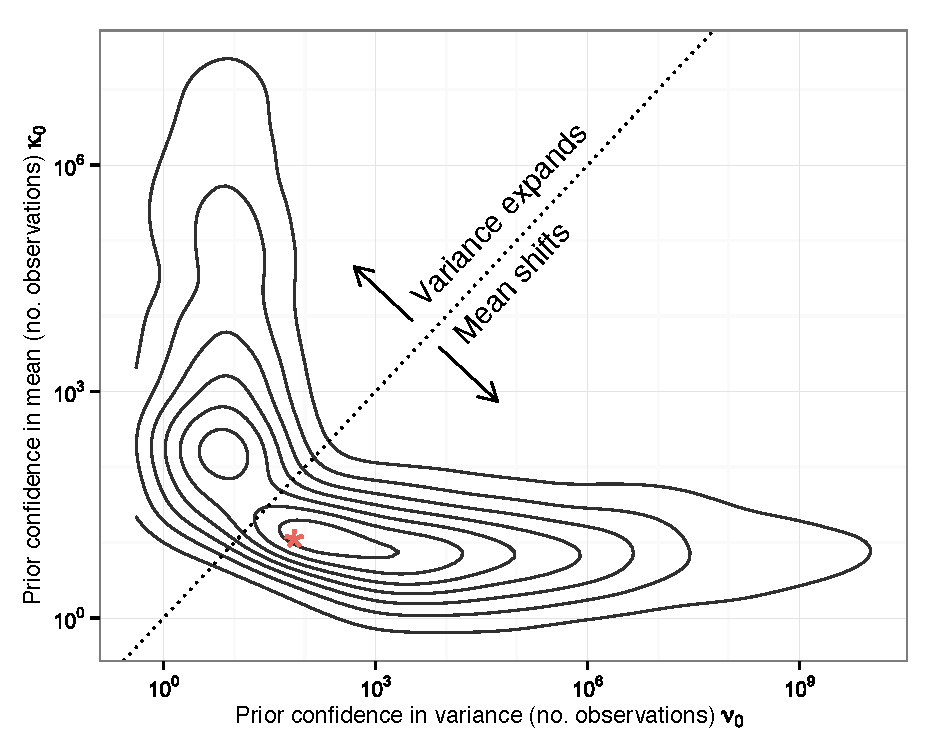
\includegraphics[width=0.6\textwidth]{figure/vroomen-recal-64-kappa-nu-joint-posterior-contour.pdf}
    \label{fig:conf-v64-recal}
  }\\
  \subfigure[V07, sel. ad., 64]{
    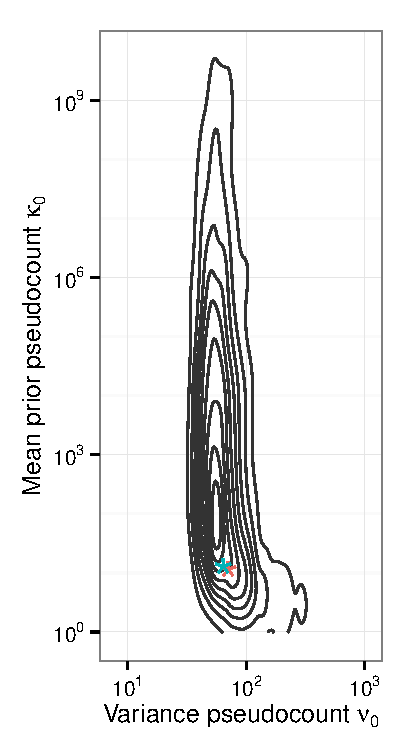
\includegraphics[width=0.1875\textwidth]{figure/vroomen-selad-64-kappa-nu-joint-posterior-contour.pdf}
    \label{fig:conf-v64-selad}
  }
  \subfigure[V07, simult.]{
    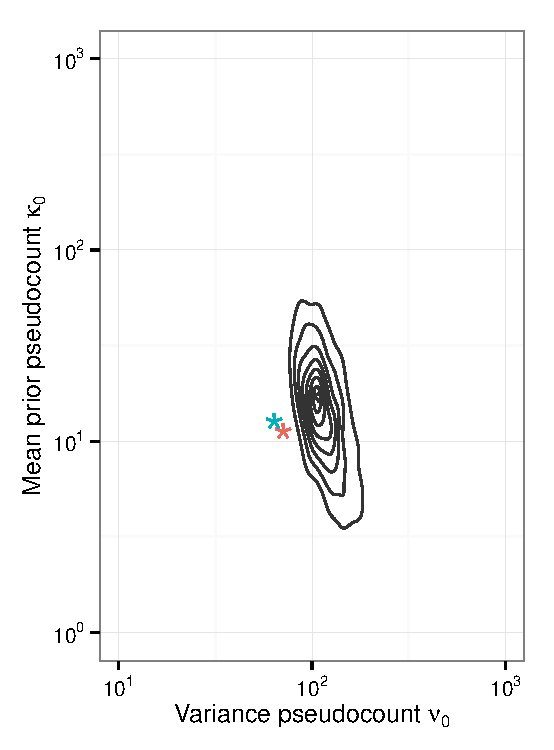
\includegraphics[width=0.252\textwidth]{figure/vroomen-both-256-kappa-nu-joint-posterior-contour.pdf}
    \label{fig:conf-v256}
  }
  \subfigure[MTurk data, simult.]{
    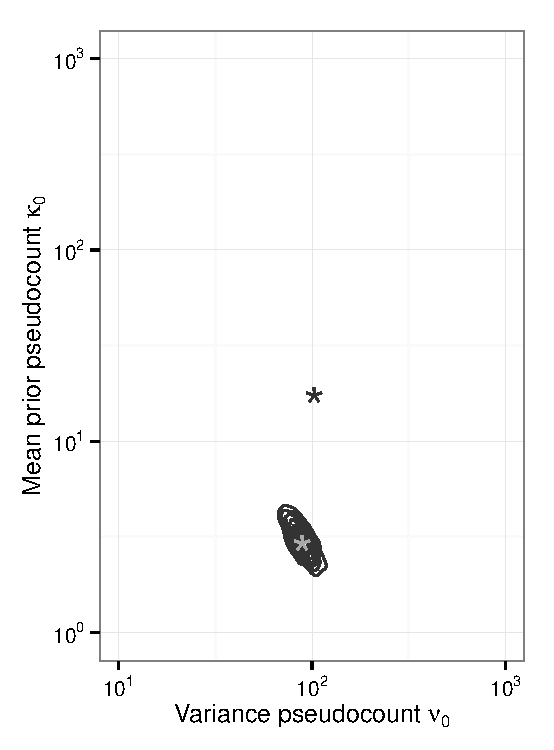
\includegraphics[width=0.252\textwidth]{figure/mturk-kappa-nu-joint-posterior-contour.pdf}
    \label{fig:conf-mturk}
  }
  \caption{MCMC-estimated joint posterior density (contours) and MAP-estimates (asterisks) of prior confidence parameters for all studies presented in the main text. Black asterisk shows MAP estimate for combined fit, and colored asterisks show earlier fits. Blue asterisk shows the MAP estimate for the selective adaptation condition, and red the recalibration condition. Panel \subref{fig:conf-v64-recal}: perceptual recalibration data from Vroomen et al. (2007) up 64 exposures (replotted for convenience). Panel \subref{fig:conf-v64-selad}: selective adaptation data from Vroomen et al. (2007) up to 64 exposures. Panel \subref{fig:conf-v256}: data from both recalibration and selective adaptation Vroomen et al. (2007) up to 256 exposures. Panel \subref{fig:conf-mturk}: data from our web-based experiment. Light grey asterisk shows MAP estimate for these fits and dark asterisk shows MAP estimates from fit to Vroomen et al. (2007) data for comparison.}
  \label{fig:confidence-hyperparam-posteriors}
\end{figure}


\section{Model assumptions}
\label{sec:model-assumptions}

In order to relate the qualitative predictions of the ideal adapter framework to the behavior of human listeners, it is necessary or convenient to make some simplifying assumptions.  Table~\ref{tab:model-assumptions} review these assumptions, whether they are justified, and if not, whether violating them leads to problems for the conclusions we reach from our modeling results. Many of them have already been introduced and discussed above.  None of these assumptions bias the results of the modeling towards better fits.  If anything many of them make it harder for the model to fit data which violates them.

All of these assumptions are assumptions of the model, and \emph{not} the ideal adapter framework.  In particular, the assumption that all observed cues (from one category) are identically distributed goes against the basic point of the ideal adapter analysis that cue distributions change from one situation to another, but it is a necessary simplification for specifically modeling beliefs about cues in the \emph{particular} situation of a laboratory experiment.  Also, a true ideal adapter would use their prior experience with category variance and base rate category probabilities to set these for each category, but we assume they are equal for \ph b and \ph d because this is a convenient simplification which reduces the number of hyperparameters that need to be estimate to fit the model without qualitatively changing the predictions.

\nocite{Vitevitch2004,Zhu2007}

\clearpage

\begin{footnotesize}
  \linespread{1.1}

\begin{center}
\begin{longtable}{p{0.2\textwidth} | p{0.4\textwidth} | p{0.3\textwidth}}
  \caption{Assumptions of the belief updating model used to evaluate the ideal adapter framework predictions.} \label{tab:model-assumptions} \\

  Assumption & Simplification justified by data? & Problem? \\ \hline
  \endfirsthead

  \multicolumn{3}{c}{{\bfseries \tablename\ \thetable{} -- continued from previous page}} \\
  Assumption & Simplification justified by data? & Problem? \\ \hline
  \endhead

Independently and identically distributed cues.
  &  No: non-stationarity/lack of invariance means cue distributions are different.
  &  Not for modeling first block adaptation in the lab (listeners seem to assume that they're in a totally new situation).
\\ \hline
Equal prior variances
  &  Probably not, a priori. Also, pilot simulations show that asymmetrical prior variance leads to an overall increase or decrease in the proportion of \ph b responses \emph{regardless} of the exposure category, and the same pattern shows up in the data.
  &  Not when using the aftereffect measure, which effectively controls for changes in overall rate of /b/ responses.
\\ \hline
Equal prior probability of \ph b vs. \ph d
  &  No.  /b/ is more than twice as likely as /d/ in this context \autocite{Vitevitch2004}.  However, listeners make roughly equal numbers of /b/ and /d/ responses during pre-test so they could infer that /b/ and /d/ are equally likely in this task.
  &  No, based on pilot simulations there's no qualitative difference.
\\ \hline
No change in beliefs about prior probabilities
  & Unclear.
  & No.  When confidence in prior probability is included as a free hyperparameter, it's always inferred to be very high (no change).
\\ \hline
Labeled data (supervised adaptation)
  &  Yes.  Listeners can classify the ambiguous audio-visual stimuli nearly perfectly (98\%), and they can't discriminate between ambiguous and prototypical audio-visual adaptor from the same category \autocite[52\% on an ABX task;][]{Vroomen2004}.
  &
\\ \hline
Only labeled data counts for adaptation
  &  Unclear. Listeners can adapt to shifted distributions without additional information \autocite{Munson2011}.  Fully optimal ideal adapter predicts beliefs should be partially updated \eqref{eq:18}, but depends on tracking the full posterior distribution for all previous observations which may be psychologically implausible.
  &  Probably not: doubling the number of test trials doesn't change adaptation.  Other category learning studies suggest that when there are many unlabeled training items, they have little influence on later behavior \autocite{Zhu2007}, but it's a question for future work.
\\ \hline
Adaptation to integrated audio and visual cues
  &  Maybe, see main text for discussion. %Section~\ref{sec:audio-visual-cue}
  &  Probably not.  There are other reasons why the ambiguous audio-visual adaptor might not be perceived as ambiguous for the purposes of adaptation as discussed above.%in Section~\ref{sec:import-audio-visu}.
\\ \hline
Normal distributions for cues; Normal-$\chi^{-2}$ parameter distributions
  &  Normal cue distributions are a common assumption in computational modeling, and using a conjugate prior is a natural, convenient choice.
  &  No: any distribution that is informationally efficient (has few enough effective parameters) would predict the same kind of rapid/stable adaptation.
\\ \hline
Order of trials doesn't matter (exchangeability)
  &  No: \textcite{Kraljic2008a} and carry over effects between blocks observed in our own data and \textcite{Vroomen2007} (see Supplementary Material for discussion).%(Section~\ref{sec:carry-over-effects}).
  &  No: when modeling just the first block of exposure to simple cue statistics, exchangeability is probably reasonable.
\\ \hline
Independence of prior beliefs about different categories
  &  No.  For instance: vowel F1 means are all higher for female vs. male talkers, which introduces positive correlations between the means across talkers \autocite{Hillenbrand1995}.
  &  Probably not, especially when prior beliefs are weak, as we have argued is expected in laboratory studies with unusual speech (and is supported by the estimates of weak prior confidence).
\\ \hline

\end{longtable}
\end{center}
\end{footnotesize}
